\documentclass[12pt]{article}
\usepackage{sbc-template}
\usepackage[utf8]{inputenc}
\usepackage[portuguese]{babel}
\usepackage{lipsum} 
\usepackage{graphicx,url}
\usepackage{amsfonts,amsmath,bm,bbm}
\usepackage{natbib}
\usepackage{esvect}
\usepackage[colorlinks=true, allcolors=blue]{hyperref} 

\sloppy

\title{Weighted Amplitude Transition Graph: Distinguishing amplitude information between time series}

\author{Eduarda T.\ C.\ Chagas\inst{1}}


\address{
  Departamento de Ciência da Computação\\
  Universidade Federal de Minas Gerais (UFMG) -- Belo Horizonte, MG -- Brazil
  \email{eduarda.chagas@dcc.ufmg.br}
}

\begin{document}

\maketitle

\section{Introduction}\label{Intro}

Diante dos atuais métodos que nos fornecem informações da estrutura ordinal da série, recentes trabalhos sugerem uma ponderação no cálculo das frequências relativas para padrões ordinais com variância de amplitude diferentes, fazendo-os contribuir de maneira diferente no valor final de PE e assim incorporando a informação de mudança de amplitude dentro de um determinado conjunto de dados~\citep{Fadlallah2013Weightedpermutation}.

No entanto, analisando os atuais métodos ainda percebemos uma grande falha em suas definições: não consideram a diferença de amplitude presente em diferentes séries temporais, ponderando-as de maneira semelhante no cálculo do valor final de suas probabilidades.
Logo, dados com diferentes amplitudes porém com dinâmica de variâncias similares não são discriminados, perdendo importantes informações acerca da dinâmica do sistema.

Para contrabalançar esses fatos, propomos uma modificação do atual procedimento dos grafos de transição de padrões ordinais para incorporar informações significativas das séries temporais, tendo como principal motivação salvar informações úteis de amplitude transportadas pelo sinal.

Avaliamos nossa técnica propondo uma uma nova metodologia de caracterização de regiões em texturas de imagens \texttt{SAR}. 
Ao receber uma textura realizamos o processo de linearização aplicando \textit{space filling curves} e por meio do grafo de transição de amplitude ponderada usamos o poder discriminatório da Teoria da Informação para realizar a caracterização.

O artigo foi dividido do seguinte modo: 
Na seção~\ref{OP}, introduzimos o conceito de simbolização em padrões ordinais em séries temporais, descrevendo o método de Bandt \& Pompe; 
na seção~\ref{OPTG}, apresentamos os grafos de transição de padrões ordinais;
na seção~\ref{WATG}, propomos a nossa técnica de ponderação do grafo de transição de padrões ordinais pela amplitude;
na seção~\ref{HC}, relatamos os descritores da Teoria da Informação utilizados ao longo deste trabalho;
na seção~\ref{SAR}, mostramos os resultados obtidos na caracterização de regiões em imagens \texttt{SAR};
e por último na seção~\ref{Conclusion}, concluímos o trabalho.

\section{Ordinal Patterns representations - (OP)}\label{OP}

A representação por padrões ordinais foi introduzida por~\cite{Bandt2002Permutation}, sendo utilizada como método para mensurar o grau de complexidade de dados provenientes de séries temporais através de descritores da Teoria da Informação. 
Tratando-se de um método não paramétrico, a formação de padrões ordinais por Bandt-Pompe consiste de uma abordagem simples, imune a efeitos de contaminação de ruídos, invariante a transformações monótonas não lineares e por considerar a causalidade temporal dos dados, revela detalhes importantes da estrutura ordinal da série temporal~\citep{Larrondo2006Random}.

Seja uma série temporal a tempo discreto $\mathbb{X} = (x_1, x_2, \dots, x_T)$ com comprimento $T$, os símbolos $\mathbb{X}_t^{m,\tau}$ realizados em cada instante $t = 1, \dots, T-(m-1)\tau$ são dados por uma dimensão de incorporação $m \in \mathbb{N}$ e tempo de atraso (delay) entre os padrões $\tau \in \mathbb{N}$: 
\begin{equation}
    \mathbb{X}_t^{m,\tau} = (x_{(t-1)+\tau}, x_{(t-1)+\tau+1},\ldots, x_{(t-1)+\tau+(m-1)}).
\end{equation}

O conjunto de padrões ordinais $\pi = \{\pi_t^m: t = 1, \dots, T-(m-1)\tau\}$ são obtidos pelo mapeamento $\mathbb{X}^{m,\tau}_t \mapsto \pi^m$ realizado através do processo de permutação dos elementos, de tal forma que estes estejam ordenados de forma crescente~\citep{Ravetti2014noise}:

$$ x_{(t-1)+\tau} \leq x_{(t-1)+\tau+1} \leq \ldots \leq x_{(t-1)+\tau+(m-1)}. $$ 

A distribuição de probabilidade de Bandt-Pompe consistirá no cálculo da frequência relativa dos símbolos da série diante das $m!$ possíveis permutações dos padrões $\{\pi_t^m\}_{t=1}^{m!}$, sendo definida como:

\begin{equation}
    p(\pi_i^m) = \frac{\#\left \{t | t = 1, \dots, T-(m-1)\tau; \mathbb{X}_t^{m,\tau} do \hspace{.2cm} tipo \hspace{.2cm} \pi_i^m\right \}}{T- (m-1)\tau},  
\end{equation}

satisfazendo as condições $p(\pi_i^m) \ge 0$ e  $\sum_{i=1}^{m!} p(\pi_i^m) = 1$.

\section{Ordinal Patterns Transition Graph -- (OPTG)}\label{OPTG}

Procurando extrair características intrínsecas do fenômenos geradores das séries temporais, os grafos de transição de padrões ordinais surgem como uma etapa adicional na análise não-paramétrica por descritores da Teoria da Informação.

Sendo $\Pi$ a sequência de símbolos obtidos por uma dada série $\mathbb{X}_t^{m,\tau}$, o grafo $\vec{G}_{\pi} = (\vec{V}, \vec{E})$ nos informa as transições entre dois padrões ordinais consecutivos ao longo do tempo $t$.
Nesta nova representação, os padrões $\{\pi_t^m\}_{t=1}^{m!}$ correspondem aos vértices do conjunto $\vec{V} = \{ v_{\pi_i}:i = 1, \dots, m!\}$ e as arestas $\vec{E} = \{(v_{\pi_i}, v_{\pi_j}): v_{\pi_i}, v_{\pi_j} \in V\}$ nos indicam a ocorrência sequencial de dois padrões ordinais no conjunto de dados analisado.

Duas abordagens são consideradas em relação ao peso das arestas na literatura: alguns autores empregam arestas não ponderadas~\citep{McCullough2015lagged, Kulp2016ordinal} representando apenas a existência de tais transições, enquanto outros aplicam a frequência das transições como pesos~\citep{Sorrentino2015periodic, Zhang2017ConstructingOP}.


Os pesos $\mathbb{W} = \{w_{v_{\pi_i}, v_{\pi_j}}: v_{\pi_i}, v_{\pi_j} \in V\}$  atribuídos a cada aresta retratam as probabilidades de transição entre dois determinados padrões  $(v_{\pi_i}, v_{\pi_j})$ calculados através de suas respectivas frequências relativas, ou seja:

\begin{equation}
    w_{v_{\pi_i}, v_{\pi_j}} = \frac{|\Pi_{\pi_i,\pi_j}|}{m-1},
\end{equation}

onde $|\Pi_{\pi_i,\pi_j}|$ nos informa o número de transições do padrão $\pi_i$ para o padrão $\pi_j$ e $\sum_{v_{\pi_i}, v_{\pi_j}}w_{v_{\pi_i}, v_{\pi_j}} = 1$.

\section{Weighted Amplitude Transition Graph -- (WATG)}\label{WATG}

Nos referimos a esse procedimento como grafo de transição de amplitude ponderada (WATG) e resumimos nas etapas a seguir. 

Primeiramente, cada série temporal $\mathbb{X}$ deverá ser normalizada entre o valores $0$ e $1$, uma vez que estamos gerando uma métrica de comparabilidade de diferentes conjuntos de dados.

Cada vetor $\mathbb{X}^{m, \tau}_t$ será associado com um valor de peso $\beta_t$, indicando a sua amplitude. 
Tal valor será dado por meio da maior diferença entre oos seus elementos, como podemos ver a seguir:

\begin{equation}
    \beta_t = max(x_i - x_j)
\end{equation}

onde $x_i, x_j \in \mathbb{X}^{m, \tau}_t$.

Tradicionalmente, o grafo de transição atribui peso uniforme para cada transição entre os padrões e normaliza o resultado obtido dividindo pelo total de transições.
Nesta modificação, os pesos $w_{v_{\pi_i}, v_{\pi_j}}$ atribuídos a cada aresta retrata a diferença de amplitude observada na transição.
Logo, temos que:

\begin{equation}
    w_{v_{\pi_i}, v_{\pi_j}} =  \sum_{i : \{\mathbb{X}^{m,\tau}_t \mapsto \pi_i\}} \sum_{j : \{\mathbb{X}^{m,\tau}_t \mapsto \pi_j\}} |\beta_i - \beta_j| .
\end{equation}

Dessa forma, a distribuição de probabilidade retirada do grafo de transição de amplitude ponderada é dado do seguinte modo:

\begin{equation}
    \left\{\begin{array}{l}
        \lambda_{v_{\pi_i}, v_{\pi_j}} = 1, se \hspace{.2cm} (v_{\pi_i}, v_{\pi_j}) \in \vec{E} \\
        \lambda_{v_{\pi_i}, v_{\pi_j}} = 0, caso \hspace{.2cm} contr\acute{a}rio.
        \end{array}\right.
\end{equation}

\begin{equation}
    p(\pi_i, \pi_j) = \frac{\lambda_{v_{\pi_i}, v_{\pi_j}} . w_{v_{\pi_i}, v_{\pi_j}}}{\sum_{v_{\pi_a}, v_{\pi_b}} w_{v_{\pi_a}, v_{\pi_b}}}.
\end{equation}

Note que as condições $p(\pi_i, \pi_j) \ge 0$ e $\sum_{\pi_i, \pi_j} p(\pi_i, \pi_j) = 1$ são plenamente satisfeitas.

Desse modo, séries com amplitudes uniformes possuem arestas com probabilidades de ocorrência bem distribuídas ao longo do grafo e aquelas com pequena amplitude e grandes picos possuem arestas com probabilidades de ocorrência muito maiores que as demais presentes.

\section{Informational Causal Entropy-Complexity Plane}\label{HC}

A Entropia mede o desordem ou a imprevisibilidade de um sistema caracterizado por uma função de probabilidade $\mathbb{P}$.
Seja, $\mathbb{P} = \{p_{(\pi_1, \pi_1)}, p_{(\pi_1, \pi_2)}, \dots, p_{(\pi_{m!}, \pi_{m!})}\}$ o a distribuição de probabilidade retirada do grafo de transição de amplitude ponderada da série temporal $\mathbb{X}$, a entropia de Shannon será dada por:

\begin{equation}
H(\mathbb{P}) = -\sum_{i=1}^{(m!m!)} (\log p_i) p_i.
\label{eq:Entropia}
\end{equation}

A capacidade da entropia de capturar propriedades do sistema é limitada, logo se faz necessário a utilização da mesma em conjunto de outros descritores para assim realizar uma análise mais completa.
Outras medidas interessantes são distâncias entre a função de probabilidade $\mathbb{P}$ e uma medida de probabilidade que descreva um processo não informativo, tipicamente a distribuição uniforme.

A distância de Jensen-Shannon à distribuição uniforme $ \mathbb{U} = (\frac{1}{m!m!},\dots,\frac{1}{m!m!})$ consiste de uma medida de quão similar a dinâmica subjacente está de um processo sem informação nenhuma, sendo calculada como se dá a seguir:

\begin{equation}
D(\mathbb{P}, \mathbb{U}) = \sum_{i=1}^{(m!m!)} \Big(p_i \log\frac{p_i}{u_i} +
u_i \log\frac{u_i}{p_i}
\Big).
\end{equation}

Inversamente à entropia, a complexidade estatística procura encontrar estruturas de interação e dependência entre os elementos de uma dada série, tratando-se de um fator extremamente importante no estudo de sistemas dinâmicos.

Essa propriedade é definida por meio da fórmula desenvolvida por Lopèz-Ruiz, Mancini e Calbet, onde uma Entropia e uma Distância, também chamada de desequilíbrio, podem ser combinadas no atributo Complexidade Estatística para aumentar o seu poder de descrição~\citep{Feldman2008information,Feldman1998Statistical,Lopez1995statistical}:

\begin{equation}
C(\mathbb{P}, \mathbb{U}) = H(\mathbb{P}) D(\mathbb{P}, \mathbb{U}).
\end{equation}

Cada série temporal poderá então ser descrita por um ponto $(H(\mathbb{P}), C(\mathbb{P}, \mathbb{U}))$.
O conjunto de todos os pares $(H(\mathbb{P}), C(\mathbb{P}, \mathbb{U}))$ para qualquer série temporal descrita por padrões de comprimento $m$ jaz em um subconjunto compacto $\mathbbm R^2$: o plano Entropia-Complexidade. 
Por intermédio de tal ferramenta é possível descobrir a natureza da série, determinando se esta corresponde a uma sequência caótica, estocástica ou determinística, analisando o seu comportamento, visto que estes possuem dinâmicas diferentes.

\section{Classification SAR regions}\label{SAR}

Neste trabalho propomos uma nova metodologia de caracterização de imagens \texttt{SAR}. 
Ao receber uma textura realizamos o processo de linearização aplicando \textit{space filling curves} e por meio do grafo de transição de amplitude ponderada usamos o poder discriminatório da Teoria da Informação para realizar a caracterização, usando o plano Entropia-Complexidade em diferentes regiões extraídas de texturas provenientes de imagens \texttt{SAR}.

As \textit{space filling curves} foram vistas pela primeira vez em~\cite{Nguyen1982SpaceFC}, transformando uma textura em um sinal unidimensional.
Quando usadas como métodos de varredura de uma imagem, tais funções conseguem preservar bem as propriedades eminentes da correlação espacial dos pixels, embora não forneçam um poder discriminatório suficiente para classificar texturas naturais~\citep{Lee1994Texture}. 

Assumindo que uma imagem é uma grade $N \times N$ de pixels, onde $N$ é uma potência de $2$, temos: 

\newtheorem{mydef}{Definição}
\begin{mydef}
    Uma varredura da imagem é uma função bijetora $f: \mathbb{N} \times \mathbb{N} \to \mathbb{N}$ no conjunto de pares ordenados $\{(i,j) | 1\leq i,j \leq N\}$, que denota os pontos no domínio, para o intervalo fechado de inteiros $\{1, \dots, N^2\}$. Equivalentemente, a imagem é codificada usando a varredura $f$ nas intensidades de pixel na ordem $P_{f^{-1}(1)}, P_{f^{-1}(2)}, \dots, P_{f^{-1}(N^2)}$, onde $P_{(i,j)}$ representa a intensidade do pixel da coluna $i$ e linha $j$.
    \label{def:CurveFilling}
\end{mydef}

As \textit{space filling curves}, como as técnicas de varredura \texttt{raster-1}, \texttt{raster-2} e \texttt{Hilbert} são caracterizadas pela definição~\ref{def:CurveFilling}, fornecendo uma função adequada $f$. 
Como também pode ser observado pela definição~\ref{def:CurveFilling}, as curvas nos impõe a condição de que cada pixel seja visitado apenas uma vez.
Neste trabalho, demos mais atenção ao resultado da caracterização obtida por meio da curva de \texttt{Hilbert}. 


Amplamente utilizadas no reconhecimento de características e padrões geográficos, imagens de radar de abertura sintética (\texttt{SAR}) são ricas em informações de textura. Para esta análise, três imagens \texttt{SAR} com diferentes regiões foram usadas, são elas:

\begin{itemize}
    \item Parque Nacional Sierra del Lacandon, Guatemala (adquirido em 10 de abril de 2015), disponível em \url{https://uavsar.jpl.nasa.gov/cgi-bin/product.pl?jobName=Lacand_30202_15043_006_150410_L090_CX_01#dados};
    \item Regiões oceânicas do Cabo Canaveral (adquirido em 22 de setembro de 2016);
    \item Área urbana da cidade de Munique, na Alemanha (adquirido em 5 de junho de 2015).
\end{itemize}

Um total de 160 amostras foram consideradas durante a investigação, sendo 40 amostras de cada categoria de regiões, são elas: regiões florestais da Guatemala; regiões oceânicas de Cape Canaveral com comportamento 1; regiões oceânicas de Cape Canaveral com comportamento 2 e regiões urbanas da cidade de Munique. Para ilustrar melhor o conjunto de amostras gerado, a figura~\ref{fig:RegioesSAR} exemplifica cada uma das categorias presentes.

\begin{figure}[!h]
\centering
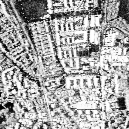
\includegraphics[width=.23\linewidth]{Figures/munichUrban.png}
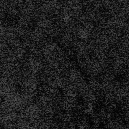
\includegraphics[width=.23\linewidth]{Figures/Cape1.png}
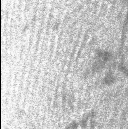
\includegraphics[width=.23\linewidth]{Figures/Cape2.png}
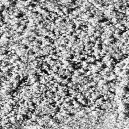
\includegraphics[width=.23\linewidth]{Figures/guatemalaflorest.png}
\caption{Tipos de regiões analisadas: (a) Regiões urbanas; (b) Região Oceânica Tipo 1; (c) Região Oceânica Tipo 2 e (d) Regiões Florestais.}\label{fig:RegioesSAR}
\end{figure} 

As imagens usadas neste experimento são resultados da banda HHHH \texttt{SAR} e cada amostra é representada por uma sub-imagem de $128 \times 128$.
Uma vez que o processo de simbolização é invariante a 
transformações monótonas e efeitos de contaminação, alterações de contraste não são capazes de provocar mudanças nos resultados finais obtidos pelos descritores. Desse modo, os diferentes tipos de regiões oceânicas considerados nesse estudo foram estudados como uma única classe mais geral.

Dados resultantes de sensoriamento remoto possuem uma característica peculiar que justifica a aplicação neste presente artigo: As intensidades de uma imagem e consequentemente a diferença de amplitude nas classes de dados depende das propriedades do alvo que estamos analisando, devido as propriedades de retroespalhamento. 
Assim, alvos urbanos são os que costumam dar mais altos retornos, seguidos por florestas, e finalmente corpos d’água, como pode-se observar na figura~\ref{fig:AmplitudeSAR}.

Portanto, neste trabalho objetivamos representar por meio do grafo de transição de amplitude ponderada modelar essa diferença de amplitude na distribuição de probabilidade dos nossos dados.
A metodologia de análise proposta e aplicada no conjunto de dados de texturas \texttt{SAR} pode ser vista na figura~\ref{fig:WATG}.

\begin{figure}[!h]
\centering
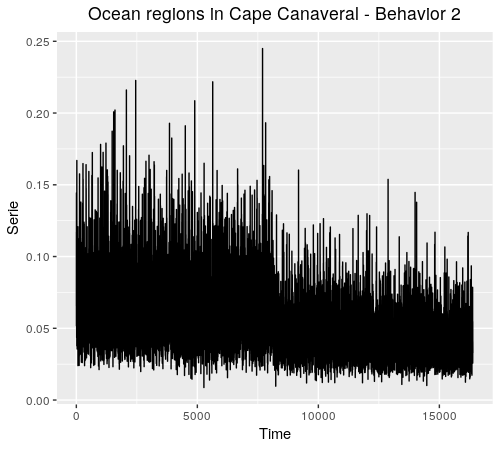
\includegraphics[width=.32\linewidth]{Figures/cape2_hilbert.png}
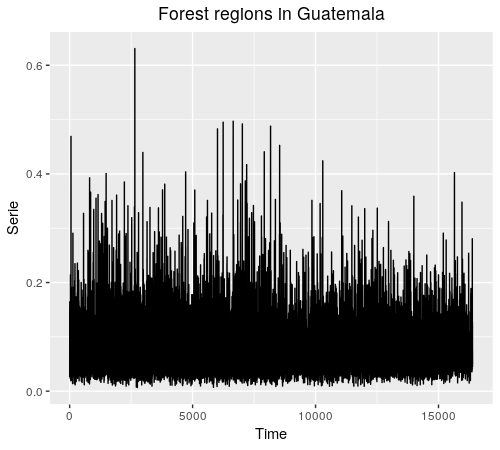
\includegraphics[width=.32\linewidth]{Figures/forestGuatemala_hilbert.png}
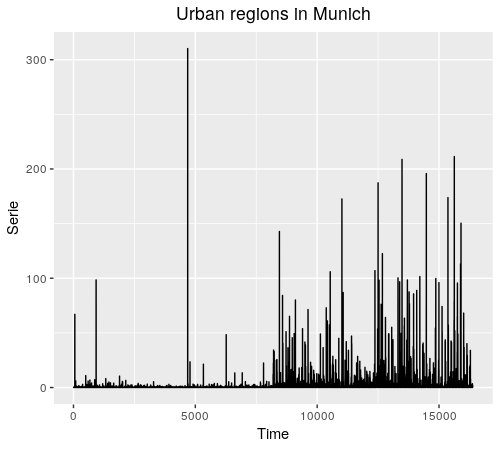
\includegraphics[width=.32\linewidth]{Figures/munich_hilbert.png}
\caption{Análise da amplitude dos diferentes tipos de regiões: (a) Região Oceânica; (b) Regiões Florestais e (c) Regiões urbanas}
\label{fig:AmplitudeSAR}
\end{figure}

Após realizada a linearização das texturas por meio da curva de Hilbert, utilizamos a técnica de janela deslizante para obter nossos símbolos, logo:

\begin{equation}
    \mathbb{X}_t^{m,\tau} = (x_{t}, x_{t+\tau},\ldots, x_{t+(m-2)\tau} ,x_{t+(m-1)\tau}).
\end{equation}

\begin{figure}[!h]
	\centering
	\vspace{-0.5cm}
	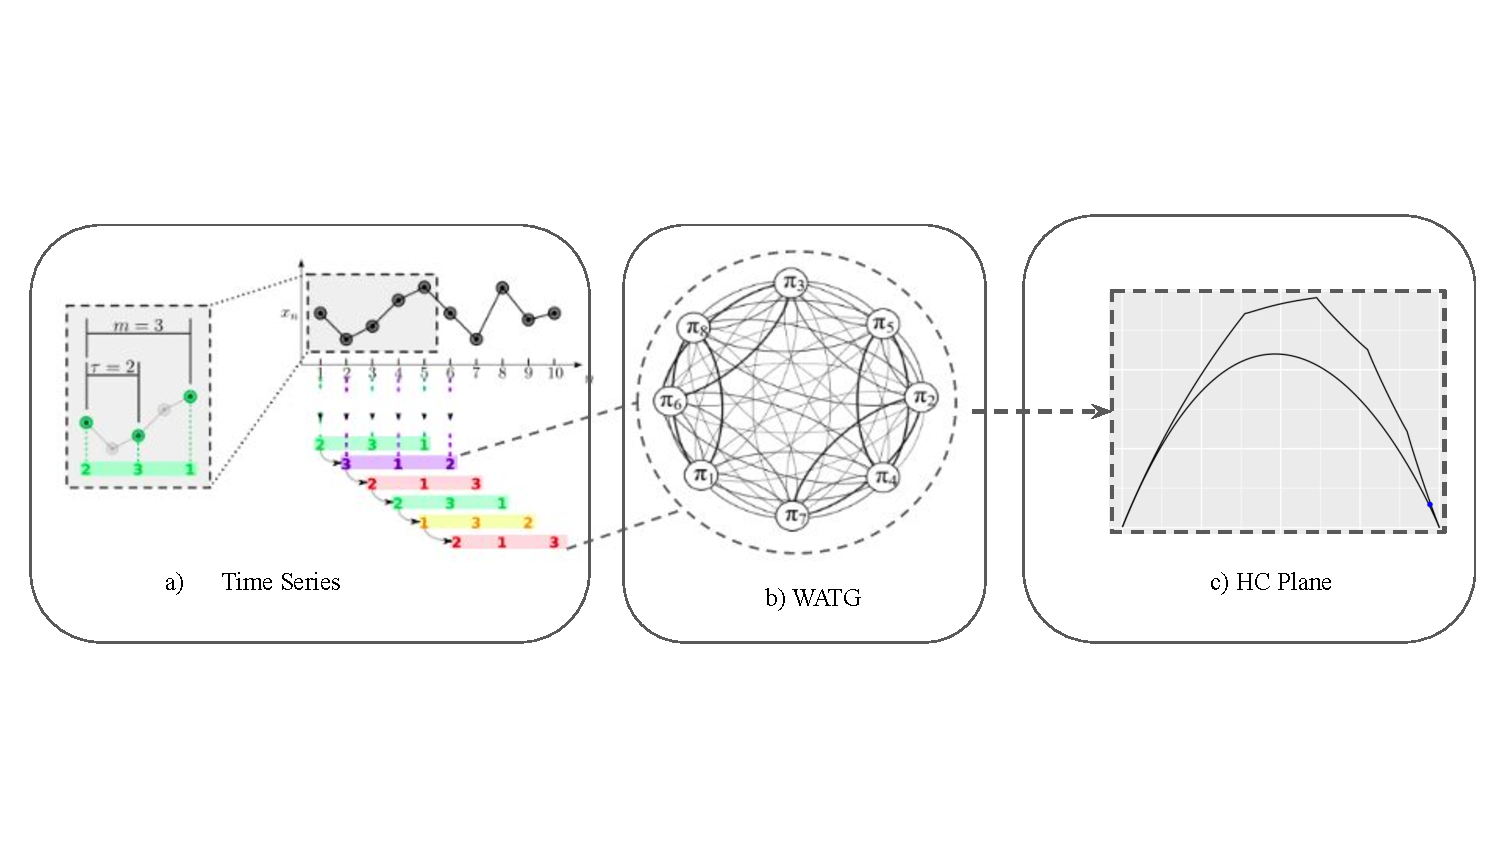
\includegraphics[scale = 0.6]{Figures/WATG.pdf}
	\vspace{-2.5cm}
    \caption{Processo metodológico aplicado na caracterização de regiões \texttt{SAR}.}
    \label{fig:WATG}
\end{figure}

Os resultados alcançados podem ser verificados na figura~\ref{fig:Regions}, onde testamos o poder do efeito da técnica sob diferentes valores de dimensão $m$ e delay $\tau$.
Uma vez que tais valores nos informam características intrínsecas da dinâmica da série nos seus domínios específicos, valores inadequados poderão vir a ocultar esse tipo de conhecimento acerca dos dados, sendo essa etapa de análise extremamente crucial. 
Como esperado, seguindo o modelo de janela deslizante, temos uma melhor caracterização quando aplicamos o delay $\tau = 1$.

\begin{figure}[!h]
	\centering
	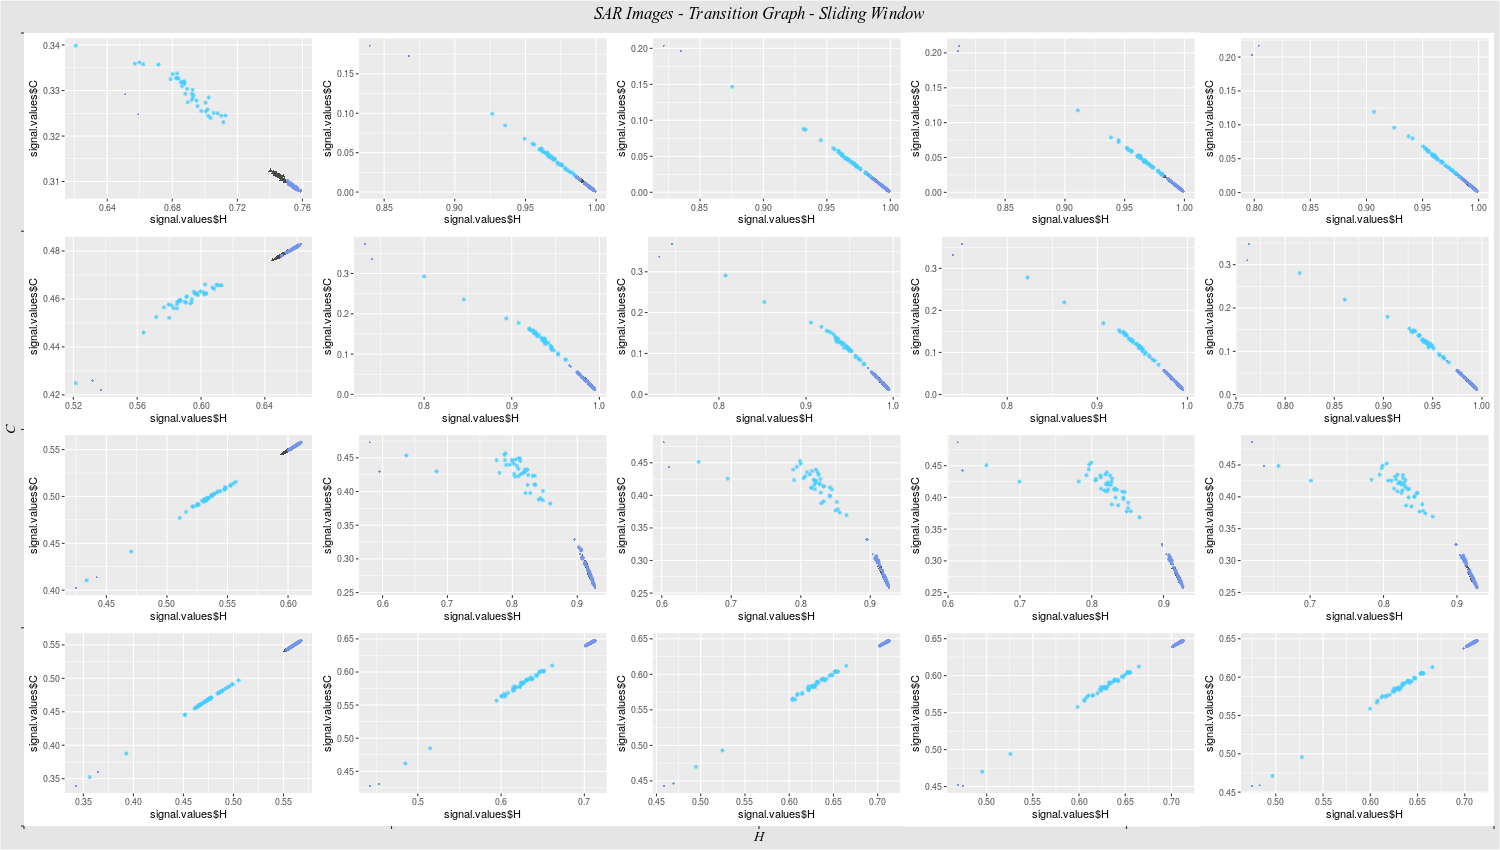
\includegraphics[width=0.9\textwidth]{Figures/transitionGraphHilbert.png}
    \caption{Caracterização resultante da aplicação da curva de \texttt{Hilbert} no WATG sobre texturas de diferentes regiões. Os gráficos evoluem horizontalmente de acordo com a dimensão $m$ escolhida e verticalmente com o delay $\tau$}
    \label{fig:Regions}
\end{figure}

\section{Conclusion}\label{Conclusion}

Neste trabalho, propomos uma nova técnica de ponderação no grafo de transição de padrões ordinais, onde agora podemos não apenas analisar a amplitude de uma dada série temporal como também dispor de uma nova métrica de comparabilidade.
A ideia se encontra em inicialmente normalizar os dados e atribuir como pesos das arestas as variações de amplitude no decorrer das transições.
Assim, quanto mais próxima a entropia $\mathbb{H}$ estiver de $0$ mais uniforme se encontrará a distribuição de probabilidade $\mathbb{P}$, nos informando que a série não possui grandes variâncias de amplitude.
Entretanto, se um série apresentar uma baixa amplitude mas possuir grandes variações (picos) ao longo do tempo, o WATG conseguirá inferir tal comportamento atribuindo um peso maior nessas transições, fazendo que a entropia $\mathbb{H}$ se aproxime de $1$.

Para testar a técnica proposta realizamos a caracterização de diferentes regiões em texturas de imagens \texttt{SAR}, que devido as propriedades de retroespalhamento em diferentes tipos de alvos, resultam após linearizadas, em séries com diferenças de amplitudes marcantes. 

Como resultados, além de separar perfeitamente áreas urbanas das demais analisadas por meio dos valores de entropia, ainda conseguimos diferenciar áreas oceânicas e florestais, através dos seus diferentes valores de complexidade estatística, que nos informa o grau de dependência temporal entre seus elementos, que agora linearizados, também nos informa sobre a dependência espacial da nossa textura.

\bibliographystyle{agsm}
\bibliography{references.bib}

\end{document}